\chapter{Formal Model of Component System Evolution}
\label{formal}
\epigraph{In theory there is no difference between theory and practice. In practice there is.}
{\textit{Jan L. A. van de Snepscheut}}
In order to facilitate the study of the component system evolution (CSE) process, a novel formal model has been developed.

Having such a model allows the definition of concepts, and enables the discussion and investigation of CSE.
The qualities that an effective and useful model should posses are described in \citep{Selic2003} as:
\begin{itemize}
  \item \textbf{Abstractness}: A model is a reduction of reality, removing or hiding detail that is irrelevant.
  \item \textbf{Understandability}: A model directly appeals to our intuition, to convey complex ideas with little intellectual effort.
  \item \textbf{Accuracy}: A model must provide a true to life representation of the modeled system.
  \item \textbf{Predictiveness}: A model must be able to be used to predict the modeled systems non-obvious, yet interesting properties.
  \item \textbf{Inexpensive}: A model must be cheaper to construct and analyze than the modeled system.
\end{itemize}
These qualities are aimed for in the CSE model presented in this chapter.

During this research, the Mancoosi project developed two novel models to describe CSE;
the Common Upgradeability Description Format (CUDF) \citep{treinen2009common} 
and the Mancoosi Optimisation Format (MOF) \citep{abate2011}.
These models where created to be used in the Mancoosi International Solver Competition (MISC)\footnote{http://www.mancoosi.org/misc/ accessed 16/4/2012},
which is held to encourage research into component system evolution problems.
To support this standard, and to be able to enter the MISC competition, a mapping from CUDF and MOF to the CSE model is necessary.
The model presented in this chapter takes a higher view of the iterative process of component system evolution (as is the focus of this research), 
where the CUDF and MOF models only look at single iteration of CSE (as was the purpose of their creation).
This means that the CSE model in its entirity cannot be mapped to the CUDF and MOF models.

The relationships between models that are used in this research to represent the CSE process are presented in figure \ref{formal.models}.
This figure shows the CSE model (1),
CUDF (2) and MOF (3), which are presented in this chapter.
In chapter \ref{implementation} the Boolean satisfiability (SAT) problem (4), and an extension to the SAT problem with psuedo-Boolean (PB) \citep{dixon2004automating} constraints (5) is described.
The CSE model is mapped to the ``SAT + PB'' model to enable an implementation to be developed to automate the evolution of a component system.
In chapter \ref{ubunutsimulation}, the Debian \citep{Barth2005} package metadata model (6) is mapped to CUDF, this enables the simulation of the evolution of an Ubuntu system.
This mapping is largely superficial as the CUDF model is based on the dpkg metadata.

\begin{figure}[htp]
\begin{center}
  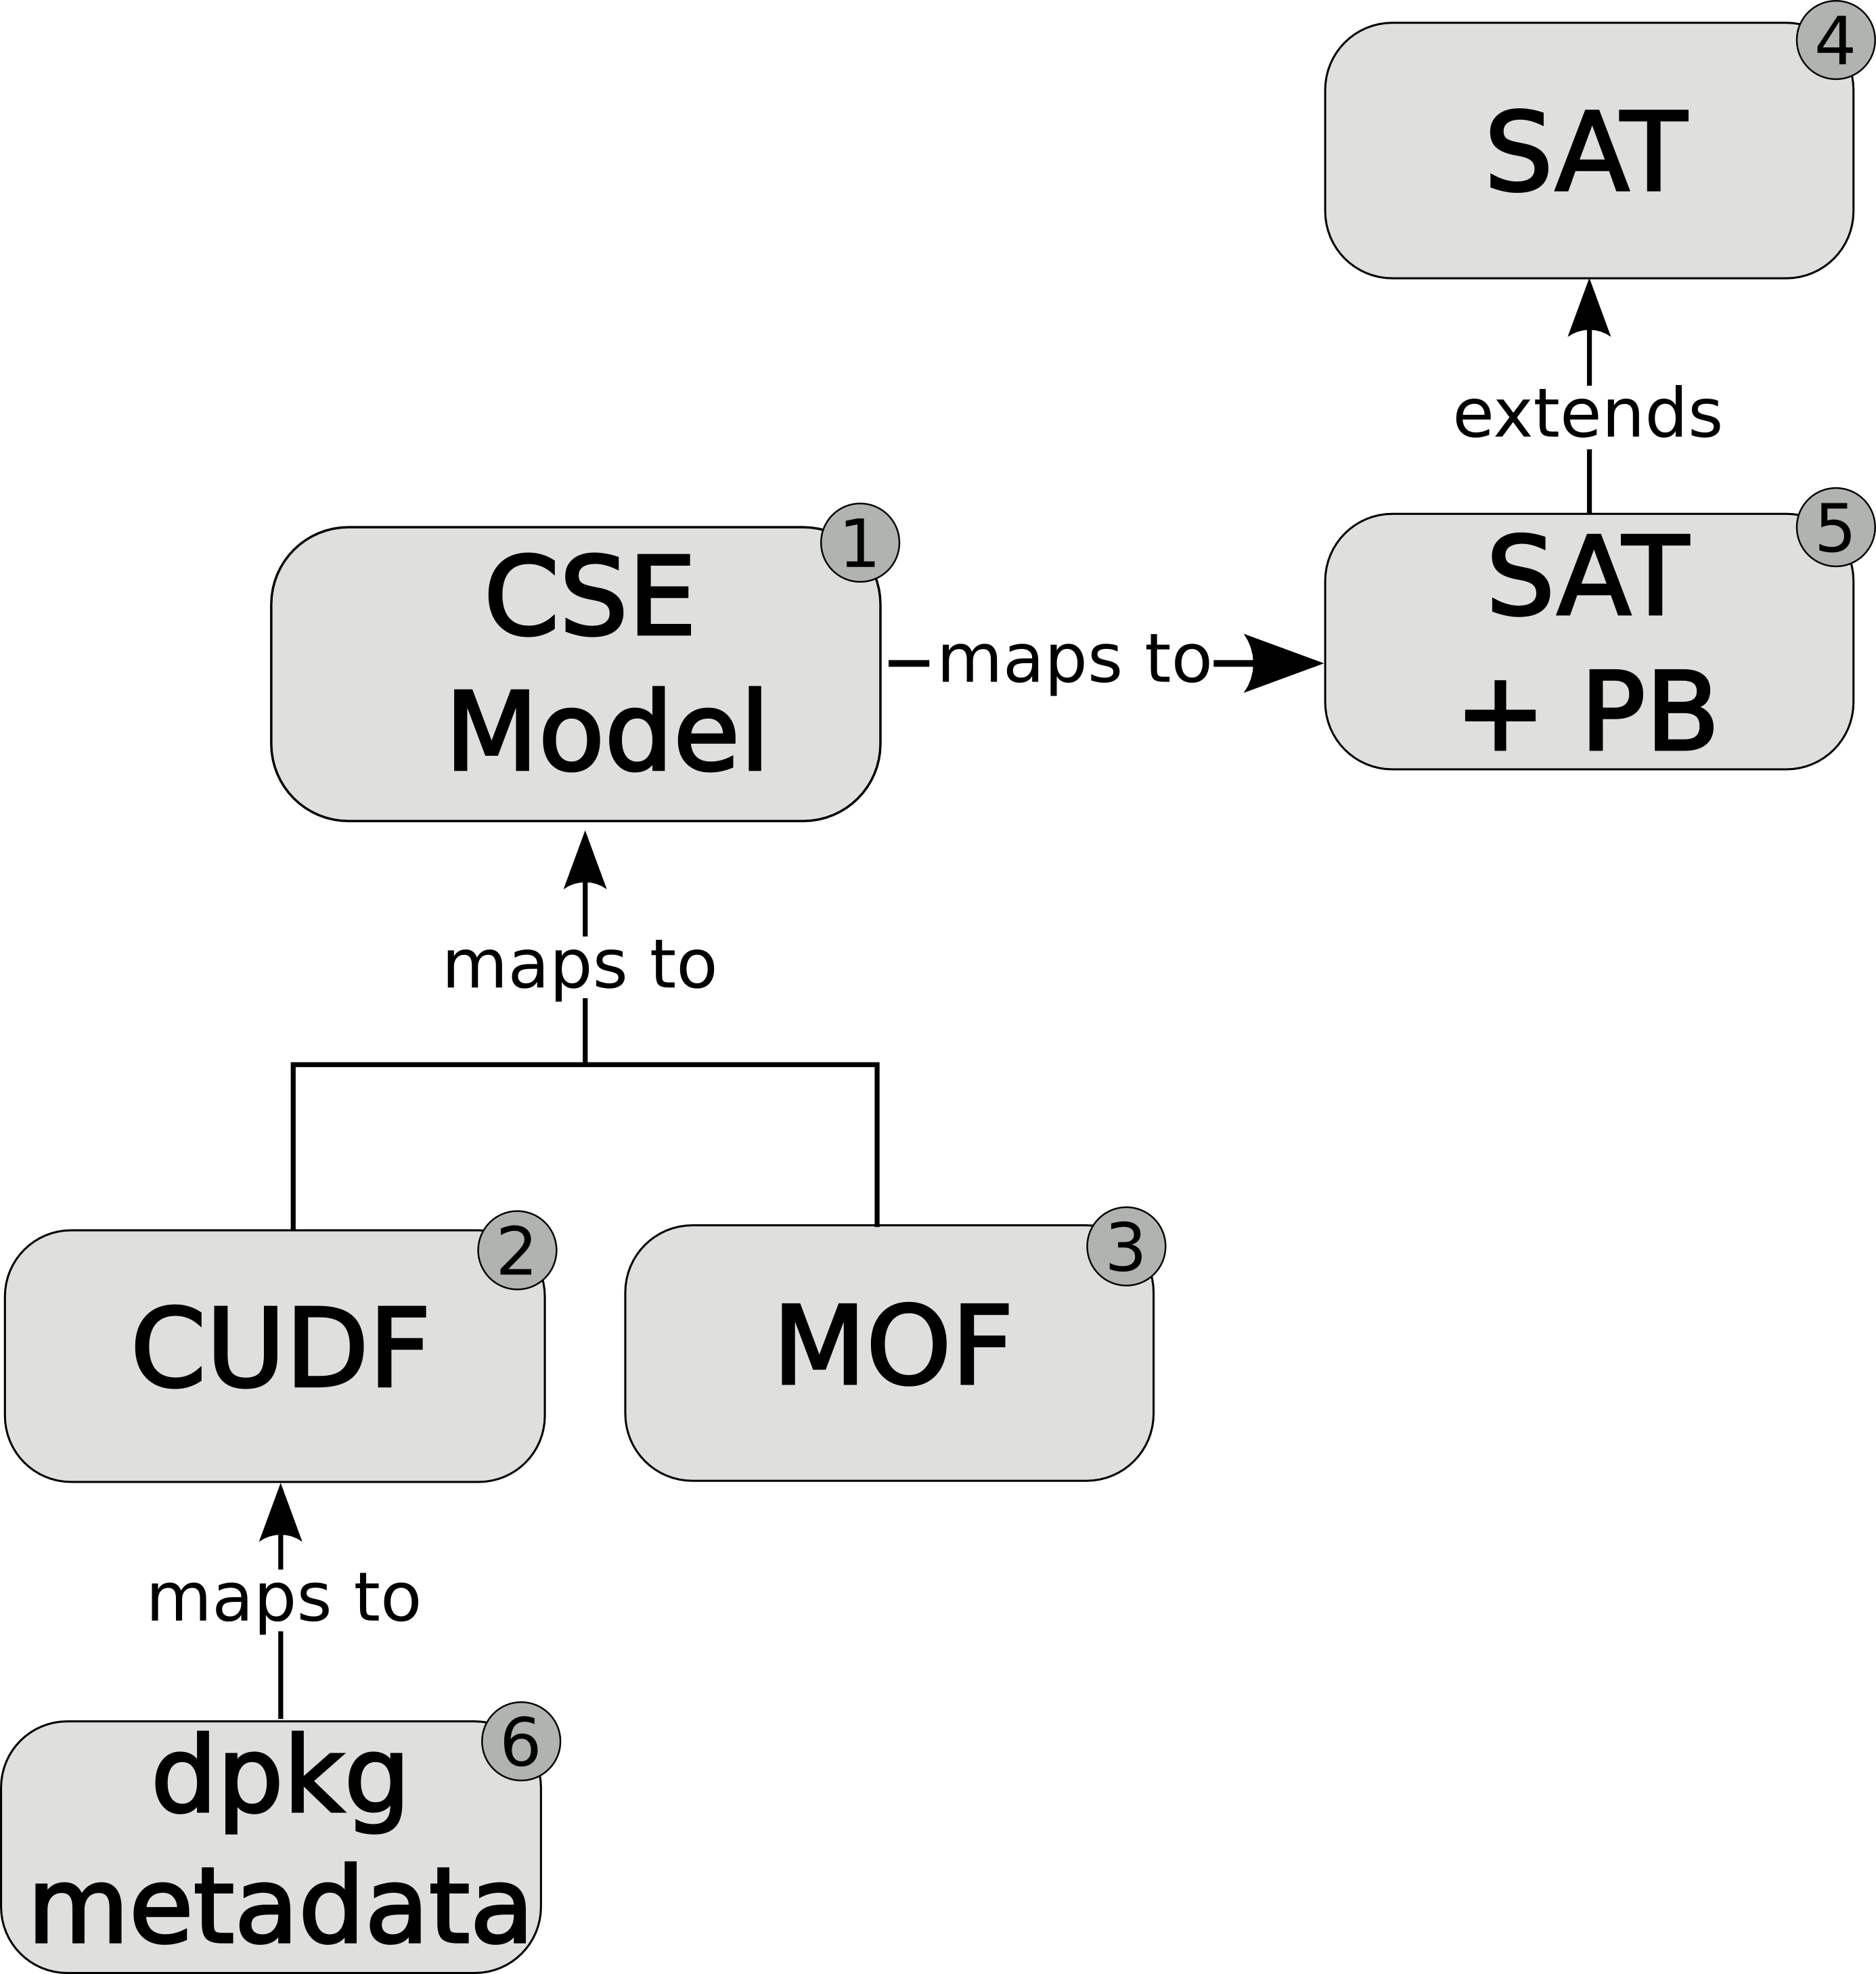
\includegraphics[width = .5\textwidth]{diagrams/models}
  \caption{Relationships between models discussed in this thesis}
  \label{formal.models}
\end{center}
\end{figure}

The CSE process is modeled as a repetitive application of evolutionary steps.
Each step satisfies a is the selection of an optimal component system that satisfies a user's request to evolve their system.
This evolution step and the CSE model are described in section \ref{formal.step}.
To define what an optimal system is, a user may have many various criteria.
Through combining these criteria lexicographically, a single measure to select a component system for an evolutionary step.
In section \ref{formal.opt} the multi-criteria problem of selecting an optimal evolution is explored.

The mapping of the CUDF and MOF models to the presented CSE model is necessary to enable the participation in the MISC competition.
It is also a useful 
Finally in section \ref{formal.cudf}, the CUDF and MOF models are mapped to the CSE model.
 
\section{Formal Model of Component System Evolution}
\label{formal.step}
Consider the problem where a user wants to install a text-editor component into their system.
For the text-editor to be functional in a component system, a spell-checker must also be in the system. 
Further assume there are three spell-checker components available.
To satisfy a users request for a text editor to be in the system, the system must evolve to a new system which includes the text-editor.
Given the text-editor requires a spell checker, at least one of these spell checkers must also be in the evolved system.

A formal model is presented in this section to represent such problems. 

\subsection{Evolution Problem}
An evolution problem defines the set of valid component systems that can be evolved to.
To define this, first the basic elements of the model must be defined.

%%%What a component is
A component is the atomic unit of component system evolution.
\begin{defs}
\label{formal.componentdef}
Let $\mathcal{N}$ be the set of names, where a name is a finite string of characters; 
let $\mathcal{V}$ be the totally ordered set of versions\footnote{Given $\mathcal{V}$ is ordered under 
$\leq$, $\leq$ is antisymmetric ($v \leq w$ and $w \leq v$ then $v = w$), transitive ($v \leq w$ and $w \leq x$ then $v \leq x$) and total ($v \leq w$ or $w \leq v$)}; 
a \textbf{component}
is an element of $\mathbb{C}$, where $\mathbb{C} = \mathcal{N} \times \mathcal{V}$.
\end{defs}
A component $a$ is then a pair $\langle n,v \rangle$, where $n$ is the component's name, and $v$ is the component's version.
The characters  $a,b,c,\ldots$ are used to denote components, $m,n,o,\ldots$ used to denote names, and $v,w,x,\ldots$ used to denote versions.

\begin{defs}
\label{formal.componentsystemdef}
A \textbf{component system} is a finite subset of components, e.g. $\alpha$ is a component system where $\alpha \subseteq_{finite} \mathbb{C}$. 
\end{defs}
The characters $\alpha,\beta,\gamma$ are used to denote component systems\footnote{In recursive component models, such as Fractal \citep{Quma2006}, 
a component system would also be a component.
That is, a component system could have elements that are themselves component systems.
This definition is not included in this model, though it may be possible to be modified to include it if required.}.

Constraints are used to restrict valid systems.
\begin{defs}
\label{formal.constraintdefs}
A \textbf{constraint} is set of component systems, e.g. $con$ is a constraint and $con \subseteq 2^{\mathbb{C}}$.
\end{defs}

Only certain types of constraints are considered in this model, these types are:
\begin{enumerate}
  \item \textbf{Exclusion}: $\neg a := \{\alpha \in 2^{\mathbb{C}} \mid a \not \in \alpha \}$ \label{formal.removeconstraint}.
  \item \textbf{Conflict}: $a \rightarrow \neg c := \{\alpha \in 2^{\mathbb{C}} \mid \mbox{if } a \in \alpha \mbox{ then } c \not \in \alpha\}$ \label{formal.conflictconstraint}.
  \item \textbf{Inclusive Disjunction}: $a_1 \vee \ldots \vee a_n := \{\alpha \in 2^{\mathbb{C}} \mid a_1 \in \alpha \mbox{ or }\ldots \mbox{ or } a_n \in \alpha\}$ \label{formal.keepconstraint}.
  \item \textbf{Dependence}: $a \rightarrow c_1 \vee \ldots \vee c_n := \{\alpha \in 2^{\mathbb{C}} \mid \mbox{if } a_1 \in \alpha \mbox{ then }  c_1 \in \alpha \mbox{ or } \ldots \mbox{ or } c_n \in \alpha\}$ \label{formal.dependencyconstraint}.
  \item \textbf{Exactly One}: $a_1 + \ldots + a_n = 1 := \{\alpha \in 2^{\mathbb{C}} \mid |\{a_1,\ldots,a_n\} \cap \alpha| = 1\}$ \label{formal.upgradeconstraint}.
\end{enumerate}
The set of constraints is restricted to these types only. 
Note, for constraint types \ref{formal.keepconstraint}, \ref{formal.dependencyconstraint} and \ref{formal.upgradeconstraint} the value of $n$ can be equal to $1$.

The vocabulary used when discussing constraints is as follows:
\begin{defs}
\label{formal.constraintdefs}
A component system $\alpha$ is said to \textbf{satisfy} a constraint $con$ iff $\alpha \in con$.
\end{defs}

\begin{defs}
An \textbf{evolution problem} $EP$ is a finite set of constraints.
\end{defs}

\begin{defs}
A \textbf{solution} to an evolution problem $EP$ is a component system  $\alpha$  that satisfies all constraints in the evolution problem, i.e. $\alpha \in con_i$ for all $con_i \in EP$.  
\end{defs}
A valid system, w.r.t. an evolution problem, is described as a solution to the evolution problem.

There can exist evolution problems that have no solution: 
\begin{defs}
An evolution problem is \textbf{unsatisfiable} if there exists no solution to it.  
\end{defs}


\subsubsection{Example}
Assume the evolution problem $EP$ is defined as the set of two constraints $con_1$ and $con_2$, i.e. $EP = \{con_1,con_2\}$.
The constraints $con_1$ is $b$ (constraint type \ref{formal.keepconstraint}), which is defined as the set of all component system with $b$ in them.
The constraint $con_2$ is $a \rightarrow c$ (constraint type \ref{formal.dependencyconstraint}), which is defined as the set of all component systems where if $a$ is included, then $c$ is included.
The component systems that satisfy both $con_1$ and $con_2$ are solutions to $EP$.
Some solutions to $EP$ are $\{b\}$, $\{a,b,c\}$ and $\{a,b,c,d\}$.

\subsubsection{Complexity of the Evolution Problem}
When investigating the complexity of an evolution problem, the observation was made that:
\begin{obs}
Finding a solution to an evolution problem is NP-complete \citep{cook1971}.
\end{obs}
This observation has been made before by \cite{Mancinelli2006} and \cite{abate2011}.
This can be shown by reducing a known NP-complete problem, called one-in-three satisfiability, to the evolution problem.
The one-in-three satisfiability problem is defined by \cite{Schaefer1978} as:
\begin{quote}
Given sets $S_1, \ldots, S_n$ each having at most 3 members, is there a subset $T$ of the members such that for each $i$, $|T \cap S_i|  =  1$.
\end{quote}

This can be reduced to an evolution problem where:
\begin{quote}
Given sets $S_1, \ldots, S_n$ each containing 3 components, and constraints $con_1,\ldots,con_n$
such that for each $i$, $S_i = \{a,b,c\}$ iff $con_i$ equals constraint $a + b + c = 1$ (constraint type \ref{formal.upgradeconstraint}).
A set of components $\alpha$ is such that for each $i$, $|\alpha \cap S_i|  =  1$ iff $\alpha$ is a solution to the evolution problem $EP = \{con_1,\ldots,con_m\}$.
\end{quote}

This reduction uses the ``exactly one'' constraint (type \ref{formal.upgradeconstraint}).
However, if this constraint type was not included into this formalism, the evolution problem would still be NP-Complete,
as one-in-three satisfiability can be reduced to a problem consisting of  constraint types \ref{formal.conflictconstraint} and \ref{formal.keepconstraint}.

\subsection{Constraints and Requests}
\label{formal.constraints}
An evolution problem is made of two sets of constraints; constraints created by the user's request to change the system, 
and constraints required for the system to be valid.

\begin{defs}
The set of \textbf{user requests} $\Delta$ is the set of all constraints, where each constraint in $\Delta$ is either:
\begin{itemize}
  \item an \textbf{installation} request of constraint type \ref{formal.keepconstraint}.
  \item a \textbf{remove} request of constraint type \ref{formal.removeconstraint}.
  \item an \textbf{*grade} request of constraint type \ref{formal.upgradeconstraint}.
\end{itemize}
\end{defs}

Consider the examples of:
\begin{itemize}
  \item an installation request $a \vee b$ is a request by the user to install component $a$ or $b$ into the system.
  \item a remove request $\neg a$ is a request by the user to remove component $a$ from the system.
  \item an *grade request $a + b = 1$ is a request by the user to include either $a$ or $b$, but not both.
\end{itemize} 

The *grade request uses the ``exactly one'' constraint (type \ref{formal.upgradeconstraint}) to represent both downgrade and upgrade requests from the user.
The intuition is that after upgrading or downgrading a component, exactly one component (that is being *graded) should be included in the system \citep{treinen2009common}.
This request does not require the name or version of the components, as that may not be the aspect being *graded.
For example, a user may want to upgrade a service that various components provide; the names and versions of the components are not related to this request.

\begin{defs}
The set of \textbf{system constraints} $\Omega$ is a set of all constraints, where each constraint in $\Omega$ is either: 
\begin{itemize}
  \item a \textbf{keep} constraint of type \ref{formal.keepconstraint}.
  \item a \textbf{dependency} constraint of type \ref{formal.dependencyconstraint}.
  \item a \textbf{conflict} constraint of type \ref{formal.conflictconstraint}.
\end{itemize}
\end{defs}

Consider the examples of:
\begin{itemize}
  \item a keep constraint $a \vee b$ is a system constraint to keep component $a$ or $b$ in the system.
  \item a dependency constraint $a \rightarrow b \vee c$ is a system constraint where if $a$ is in the system, then $b$ or $c$ must be in the system.
  \item a conflict constraint $a \rightarrow \neg b$ is a system constraint where if $a$ is in the system then $b$ must not be in the system.
\end{itemize} 

As the evolution of a component system happens over a period of time, the concept of ``time'' must be introduced to the model.
\begin{defs}
The set $T$ is the set of times, which it is strictly totally ordered under $<_{time}$, where times $t_i$ and $t_{i+1}$ in $T$ implies $t_i <_{time} t_{i+1}$
\end{defs}

At any time, there exists only a finite set of components. 
\begin{defs}
$\mathbb{C}_{t}$ is the finite set of components that exist at time $t$, $\mathbb{C}_{t} \subset_{finite} \mathbb{C}$
\end{defs}

At any point in time, the sets of system constraints and user request constraints must be with respect to the set of components that exist at that time.
\begin{defs}
Given time $t$, and the set of components $\mathbb{C}_{t}$, the set of \textbf{system constraints w.r.t. time} is $\Omega_{t}$, where $\Omega_{t} = \{con \cap 2^{\mathbb{C}_{t}} \mid con \in \Omega\}$,
and the set of \textbf{user requests w.r.t. time} is $\Delta_{t}$, where $\Delta_{t} = \{con \cap 2^{\mathbb{C}_{t}} \mid con \in \Delta\}$
\end{defs}

\begin{defs}
Given a time $t$, a \textbf{user request}, $\delta_{t}$, is a finite set of user requests at time $t$, i.e. $\delta_{t} \subseteq_{finite} \Delta_{t}$;
and a set of \textbf{system constraints}, $\omega_{t}$, is a finite set of system constraints at time $t$, i.e. $\omega_{t} \subseteq_{finite} \Omega_{t}$.  
\end{defs}

An evolution problem, $EP$, can be defined by combining a user request $\delta_{t}$ and a set of system constraints $\omega_{t}$, such that $EP = \delta_{t} \cup \omega_{t}$.

\subsubsection{Example}
Consider the system constraint $con_1$ that is defined as $a \rightarrow b \vee d$, and the user request constraint $con_2$ defined as $a$ (a singleton installation constraint).
The constraint $con_1$ can (but is not limited to) be satisfied by the component systems $\{\}$, $\{b\}$, $\{a,b\}$, $\{a,b,d\}$, and $\{a,d\}$,
and the constraint $con_2$ can (but is not limited to) be satisfied by component systems $\{a\}$, $\{a,b\}$ and $\{a,b,d\}$.

Assume that at time $t$, only the components $a$ and $b$ exist, i.e $\mathbb{C}_{t} = \{a,b\}$.
The set of all component systems at time $t$ is $2^{\mathbb{C}_{t}} = \{\{\},\{a\},\{b\},\{a,b\}\}$.
Therefore, at time $t$ component $d$ does not exist, therefore is not in $\mathbb{C}_{t}$, nor in any component system in $2^{\mathbb{C}_{t}}$.

The system constraint $con_1' \in \Omega_{t}$, is such that $con_1' = con_1 \cap 2^{\mathbb{C}_{t}} = \{\{\},\{b\},\{a,b\}\}$.
The user request constraint $con_2' \in \Delta_{t}$, is such that $con_2' = con_2 \cap 2^{\mathbb{C}_{t}} = \{\{a\},\{a,b\}\}$.

Assume a set of system constraints $\omega_{t} = \{con_1'\}$, and a user request constraints $\delta_{t} = \{con_2'\}$.
An evolution problem $\delta_{t} \cup \omega_{t}$, will have exactly one solution, the component system $\{a,b\}$.  

\subsection{Component System Evolution}
\label{formal.evo}
A component system is evolved from one system to another to satisfy an evolution problem consisting of a user request and set of system constraints.
Many evolution problems have multiple valid solutions, as evolution problems are generally under-constrained \citep{Berre2008}.
As solutions have different properties, and a user may prefer one property over another; an order over the solutions exists.  

\begin{defs}
Given a component system $\alpha$, an \textbf{evolution preference order} is a strict partial order defined w.r.t. $\alpha$,  $\prec_{\alpha} \subseteq 2^{\mathbb{C}} \times 2^{\mathbb{C}}$.
\end{defs}
A strict partial order has the properties of irreflexivity (not $\beta \prec_{\alpha} \beta$), asymmetry (if $\beta \prec_{\alpha} \beta'$ then not $\beta' \prec_{\alpha} \beta$), 
and transitivity (if $\beta \prec_{\alpha} \beta'$ and $\beta' \prec_{\alpha} \beta''$ then $\beta \prec_{\alpha} \beta''$).
The non-strict evolution preference order $\preceq_{\alpha}$ can be defined such that $\beta \prec_{\alpha} \beta'$ if and only if $(\beta \preceq_{\alpha} \beta'$ and $\beta \neq \beta')$. 

\begin{defs}
Given a component system $\alpha$, an evolution preference order w.r.t. $\alpha$ $\prec_{\alpha}$, and an evolution problem $EP$;
a component system $\beta$ is \textbf{optimal} if $\beta$ is a solution to $EP$, and there exists no other solution to $EP$ $\beta'$, such that $\beta \prec_{\alpha} \beta'$.   
\end{defs}

\begin{defs}
\label{formal.stepdef}
Given times $t_{i-1}$ and $t_i$, a component system $\alpha_{t_{i-1}}$, an evolution preference order $\prec_{\alpha_{t_{i-1}}}$, 
a user request $\delta_{t_i}$, and a set of system constraints $\omega_{t_i}$;
the \textbf{evolution step} function  $\epsilon(\alpha_{t_{i-1}},\delta_{t_i} \cup \omega_{t_i})$ returns the component system $\alpha_{t_i}$ such that:
\begin{itemize}
  \item iff the evolution problem $\delta_{t_i} \cup \omega_{t_i}$ is satisfiable, $\alpha_{t_i}$ is an optimal solution to $\delta_{t_i} \cup \omega_{t_i}$.
  \item iff the evolution problem $\delta_{t_i} \cup \omega_{t_i}$ is unsatisfiable, $\alpha_{t_i}$ equals $\alpha_{t_{i-1}}$.
\end{itemize}
\end{defs}
If the evolution problem is unsatisfiable, the evolutionary step function does not evolve the system and returns the system $\alpha_{t_{i-1}}$.
Such a situation occurs when the user requests a change that either conflicts with itself, or conflicts with the system constraints.
At the implementation level, if a request is unsatisfiable, typically a report will be returned to the user explaining why the evolution problem is unsatisfiable.
This report may also include hints to the user as to how to make the request satisfiable.
The report is not included in this model, as it is beyond the scope of the study.

Another approach to take when an evolution problem is unsatisfiable would be to return a component system that maximises the number of satisfied constraints in the user's request.
This approach, however, is made difficult because the intentions of a user's request are impossible to determine.
For example, if a user requested to install components $a$ and $b$, however either $a$ or $b$, but not both, could be installed, what component system should be returned?
Given the user request, this is a question cannot be answered as the user may of only required both $a$ and $b$, and only installing one will not satisfy the user.
Making no assumptions about the intent of the user's request is therefore the prudent approach taken in this model.

\begin{defs}
Given a series of times $t_0,\ldots,t_n$, an initial component system $\alpha_{t_0}$, 
a series of user requests $\delta_{t_1},\ldots,\delta_{t_n}$, a series of system constraints $\omega_{t_1},\ldots,\omega_{t_n}$,
and a series of evolution preference orders $\prec_{\alpha_{t_0}},\ldots, \prec_{\alpha_{t_{n-1}}}$;
the \textbf{evolution} function $\epsilon^*$ is defined as\\
$\epsilon^*(\alpha_{t_0},\langle \delta_{t_1} \cup \omega_{t_1},\ldots,\delta_{t_n} \cup \omega_{t_n} \rangle)$ $=$ $\epsilon(\epsilon(\ldots \epsilon(\alpha_{t_0},\delta_{t_1} \cup \omega_{t_1}),\ldots),\delta_{t_n} \cup \omega_{t_n})$
$=$ $\alpha_{t_n}$.
\end{defs}

This definition of the evolution function encapsulates the process of a component system evolving.
This process is the focus of this thesis.

A possible problem during this process is that a users change request could be undone with subsequent evolutions.
For example, if a user requests to install a text editor into the system, 
the user would expect that after future evolutions, the text editor will be included in the system.
This property is not explicitly stated in the model, because (as described above) it is difficult to determine a users intention with a request.

A similar problem is faced by the revision function in the domain of belief revision \citep{alchourron1985logic}.
Revision functions try to preserve consistency across a set of beliefs as new, and possibly inconsistent, information is introduced.
This is similar, as a set of previous user requests should try to remain satisfied with the component system, as the user requests to change the system.    
This problem with the evolution process is not further explored in this research, though belief revision may provide inspiration for future research.

\subsubsection{Optimal Solutions}
%%%This makes a sometimes counter intuitive complexity
The definition of the evolution function allows the observation:
\begin{obs}
Multiple evolutionary steps may produce a less optimal component system than an equivalent, single evolutionary step.
\end{obs}

This can be demonstrated with an example.
Let the evolutionary preference order select solutions with the minimum number of components altered (the symmetric difference between the solutions), 
i.e. $\beta \prec_{\alpha} \beta'$ iff $|\alpha \Delta \beta| > |\alpha \Delta \beta'|$.
Further, let:
\begin{itemize}
  \item the times $0$, $1$ and $2$;
  \item the set of components $\mathbb{C}_0 = \mathbb{C}_1 = \mathbb{C}_2 = \{a,b,c,d\}$;
  \item the system at time $0$ be $\alpha_0 = \{\}$
  \item a series of user requests be $\delta_1 = \{a\}$ and $ \delta_2 = \{c\}$
  \item the set of constraints $\omega_1 = \omega_2 = \{a \rightarrow b \vee c, c \rightarrow d\}$
\end{itemize}, 

Consider the component evolution from $\alpha_0$ to $\alpha_2$:
\begin{itemize}
  \item $\alpha_0 = \{\}$
  \item $\alpha_1 = \epsilon(\alpha_0,\delta_1 \cup \omega_1)$, given the preference order $\prec_{\alpha_0}$. $|\alpha_0 \Delta \{a,b\}| = 2$ is minimal, therefore $\alpha_1 = \{a,b\}$.
  \item $\alpha_2 = \epsilon(\alpha_1,\delta_2 \cup \omega_2)$, given the preference order $\prec_{\alpha_1}$. $|\alpha_1 \Delta \{a,b,c,d\}| = 4$ is minimal, therefore $\alpha_2 = \{a,b,c,d\}$.
\end{itemize}

Further, consider the component evolution directly from $\alpha_0$ to $\alpha_2$, where $\delta_2' = \delta_1 \cup \delta_2$:
\begin{itemize}
  \item $\alpha_0 = \{\}$
  \item $\alpha_2' = \epsilon(\alpha_0,\delta_2' \cup \omega_2)$, given the preference order $\prec_{\alpha_0}$. $|\alpha_0 \Delta \{a,c,d\}| = 3$ is minimal, therefore $\alpha_2' = \{a,c,d\}$.
\end{itemize}

In this example, the system $\alpha_2$ is less optimal than the system $\alpha_2'$ w.r.t. the order $\prec_{\alpha_0}$.
This counter-intuitive result shows that the incomplete knowledge of future user requests may effect the optimality of the evolved component system.

\section{Optimal Component System Selection}
\label{formal.opt}
%%%The formal definition of how to evolve a component system is complicated because it is a multicriteria problem
The order $\prec_{\alpha}$ is a preference order over component systems.
Systems presented in chapter \ref{background} such as Eclipse P2, apt-get, aptitude, and MPM all define multiple criteria that express the preference in their systems.

%%%A naive solution is to map all criteria to real numbers, then aggregate them through addition multiplication with weights.
A naive way to define the order $\prec_{\alpha}$, can be by defining a scoring function ($f: 2^{\mathbb{C}} \times 2^{\mathbb{C}} \rightarrow \mathbb{R}$) for each criterion. 
These functions can then be aggregated, e.g. using addition or multiplication (possibly with weights), and used to define $\prec_{\alpha}$.

For example, a function that returns the number of component that have changed between systems is defined $f_{change}(\alpha,\beta) = |\alpha \Delta \beta|$.
A function that returns the size of all components in a component system is defined $f_{size}(\alpha,\beta) = \sum \limits_{c \in \beta} size(c)$,
 where $size$ is a function that takes a component and returns its size in kilobytes.
The evolution preference order could then be defined as $\beta \prec_{\alpha} \beta'$ iff $f_{change}(\alpha,\beta) + f_{size}(\alpha,\beta) > f_{change}(\alpha,\beta') + f_{size}(\alpha,\beta')$.

%%%This has draw backs, some criteria are infinitly more important, it is not intuitive for users to weight.
Defining the evolution preference order in this manner has some drawbacks:
\begin{itemize}
  \item Information can be lost in the conversion to real numbers, e.g. the reason why a specific system was selected over another.
  \item The relationships between criteria are difficult to intuitively define, e.g. ``size $+$ change'' results in a confusing metric.
  \item Altering weights to express order over criteria does not convey meaningful information about decisions or their impact.
  For example, stating ``the size of a system is $.25$ multiplied by the change of a system'' does not convey what the implications of the weighting will be.
\end{itemize}

%%%Using composed orders
A possibly more intuitive approach to define the evolution preference order is to define a ranking function that measures a component system against an arbitrary range.
A criterion is then a ranking function and an order over its range. 
By not reducing the problem to only real numbers information can be retained about the selection of a component system.

Each criterion can then be composed together using a lexicographic order into a composite criterion.
The lexicographic composition lets an order over the preference of criteria be defined, without having to assign arbitrary weights.
This method has been used before in the MPM \citep{abate2011}.
It is the selected mechanism to define the preference order in this thesis, and is defined in this section.

\subsection{Criteria and Lexicographic Composition}
In this section a criterion and the lexicographic composition of criteria are formally defined.

\begin{defs}
A \textbf{ranking function}, $rank_{\alpha}$, is a function that ranks a component system to a range $A$ w.r.t. a component system $\alpha$, i.e. $rank_{\alpha} : 2^{\mathbb{C}} \rightarrow A$.
\end{defs}
The range $A$ could be real or natural numbers, integers, versions, components, \ldots

\begin{defs}
\label{formal.defcriteria}
A \textbf{criterion} is a tuple $\langle rank_{\alpha}, \leq \rangle$, 
where the ranking function is defined as $rank_{\alpha} : 2^{\mathbb{C}} \rightarrow A$, and $\leq$ (whose strict order is $<$) is a partial order over $A$.
\end{defs}
The order $\leq$ is a partial order; $\leq$ is reflexive ($a \leq a$), antisymmetry ($if a \leq b \text{ and } b \leq a \text{ then } a = b$), and transitive ($ \text{if } a \leq b  \text{ and } b \leq c  \text{ then } a \leq c$).

The evolution preference order is described with respect to a criterion.
\begin{defs}
\label{formal.defcrittooptimal}
The \textbf{evolution preference order} $\prec_{\alpha}$ can b defined with a criterion $\langle rank_{\alpha}, \leq \rangle$,
such that given component systems $\beta$ and $\beta'$, iff $rank_{\alpha}(\beta)$ is strictly less than ($<$) $rank_{\alpha}(\beta')$ then $\beta'$ is preferred, 
i.e. $\beta \prec_{\alpha} \beta'$ iff $rank_{\alpha}(\beta) < rank_{\alpha}(\beta')$.
\end{defs}


\begin{defs}
\label{formal.defcritlex}
The \textbf{lexicographic composition} multiple criteria into a single criterion is defined with the operator $\oplus$.
Given the component system $\alpha$, let the two criteria $crit_1 = \langle rank^1_{\alpha}, \leq_{1} \rangle$, and $crit_2 = \langle rank^1_{\alpha}, \leq_{2} \rangle$,
where the range of $rank^1_{\alpha}$ is $A_1$, and the range of $rank^2_{\alpha}$ is $A_2$.
The lexicographical composition of $crit_1$ and $crit_2$, $crit_1 \oplus crit_2$, returns the tuple $\langle rank^L_{\alpha},\leq_L \rangle$.
The range of $rank^L_{\alpha}$ is $A_1 \times A_2$, and $rank^L_{\alpha}(\beta) = \langle rank^1_{\alpha}(\beta),rank^2_{\alpha}(\beta) \rangle$.
The order $\leq_L$ (whose strict order is $<_L$) is over $A_1 \times A_2$, such that $(a,b) \leq_L (a',b')$ iff $a <_1 a'$ or $(a = a'$ and $b \leq_2 b')$.
\end{defs}

This definition leads to the observation:
\begin{obs}
The lexicographic composition of two criteria results in a criterion.
\end{obs}
That is, by using the composition $\oplus$, two criteria are lexicographically composed into a tuple $\langle rank^L_{\alpha},\leq_L \rangle$.
The order $\leq_L$ is a partial order over the range of $rank^L_{\alpha}$.
Therefore, the tuple  $\langle rank^L_{\alpha},\leq_L \rangle$ is a criterion.

This means that any number of criteria can be composed together using $\oplus$,
and resulting criterion can then be used to define the evolution preference order $\prec_{\alpha}$

\section{Common Upgradeability Description Format and Mancoosi Optimisation Format}
\label{formal.cudf}
%%%The description of the represnation of CUDF is described.
The Common Upgradeability Description Format (CUDF)\footnote{This specification was previously discussed in section \ref{background.models}, with an example shown in figure \ref{CUDFmetadata}.
}
specification presented by \citep{treinen2009common}, is a language to describe an evolution problem ($\delta_{t_i} \cup \omega_{t_i}$) and a component system ($\alpha_{t_{i-1}}$). 
The Mancoosi Optimisation Format (MOF)\footnote{http://www.mancoosi.org/misc-2011/criteria/ accessed 6/3/2012}, is a language to describe an evolution preference order ($\prec_{\alpha_{t_{i-1}}}$).
Together, CUDF and MOF provide express enough information to take a single evolutionary step.

CUDF and MOF were created to allow the comparison of various solvers in the Mancoosi International Solver Competition (MISC)\footnote{http://www.mancoosi.org/misc/ accessed 6/3/2012}.
The MISC competition was held in both 2010 and 2011,
and was entered by various state of the art, and legacy, solvers that had been created, or modified, to solve CUDF problems, with MOF preference orders.

%%%In this section\ldots
In this section the design principles and requirements of CUDF are described.
A brief overview of a CUDF document is then presented.
The CUDF specification is then mapped to our model of component system evolution.
Finally, MOF is described and is mapped to the formal optimisation model.

\subsection{CUDF Design}
\label{formal.cudfDesign}
The Mancoosi organisation is a research project committed to the improvement of the process of evolving Free and Open Source Software (FOSS) distributions.
Mancoosi looks at various problems within this domain, and have made many contributions.
One such contribution was to organise a competition between solvers of the evolution problems of FOSS systems, MISC.
This designed to encourage researchers and practitioners into researching the evolution problem.

An initial problem faced by the organisers of MISC, is that a common format was required to describe evolution problems.
The design of this format would have to follow some design principles to ensure the results would be useful.
These principles are presented in \citep{treinen2009common}, and are summarised as:

\begin{itemize}
  \item \textbf{Agnostic towards component model details}: 
  The specific component model chosen to represent the problem should be abstracted to allow many various component models to be described.  
  \item \textbf{Stay close to the original problem}: 
  The evolution problem should be the focus of the format, therefore it should not be abstracted so far as to be unrecognisable. 
  By using similar terms and syntax that already exists within the domain, the format will still directly represent the evolution problem. 
  The analysis and design of a specific problem should be able to be directly accomplished through manual investigation.
  \item \textbf{Preserve the ability for humans to inspect encoded problems}:
  This will allow greater testing and debugging, also enable the direct inspection and creation of problems by researchers.
  \item \textbf{Avoid bias towards specific implementations or techniques}:
  Specific encoding of the evolution problem, e.g. using propositional logic, or constraint programming, may create an advantage or disadvantage for a particular technique or solution.
  Since a goal of the format is to encourage the advancement of the component system evolution area, it should strive to be independent from any technique or implementation. 
  \item \textbf{Support legacy tools}:
  The comparison to tools that are already in use to solve such evolution problems, is a necessity when determining if this research is advancing the field.
  Ideally, a legacy, or current solution, should easily be able to be adapted and used with the format.
  Conversely though, the format should not stop state-of-the-art solutions from being used.
  \item \textbf{Extensible}:
  Although the format will attempt to abstract the common elements of the problem, there may still be necessary component model specific details that require inclusion.
  Also, some details are required for the optimisation of the problem, but which are not relevant to the specification of the format.
  The ability to extend the format is then required.
  \item \textbf{Transactional semantics}:
  The format should have the ability to completely represent a problem as a single unit, that can be passed to an implementation for solution.
  Also, the solution passed back should itself be a single unit, of the same format.
  This ignores aspects of the problem such as install order of the components, though this is outside the scope of the format.
  \item \textbf{Plain Text Format}:
  The use of plain text, as opposed to a binary format, will allow it to be human readable, as well as make it easier to parse and write.
  Although plain text may not be the most efficient way to encode a problem, 
  the overhead required to parse other formats may decrease the interest of researchers, or practitioners, into researching the evolution problem.
  This also aligns with the morals of the community of FOSS developers, where plain text is the universal information interchange format \citep{raymond2003art}.
\end{itemize}

The result of these design goals is the CUDF specification, presented in \citep{treinen2009common}, and described in the following sections.

\subsection{CUDF Document}
%%%Here the CUDF document is defined using text and trying to stay away from too many formalisms, just describing concepts to be used later
In this section a brief description of the CUDF format is presented.
This description is not a complete specification, but an overview of CUDF.
Some aspects of CUDF are ignored (e.g. the formal type system) as a complete redefinition of the original specification is not the goal of this section.

A CUDF document is a single plain text file, that represents all information necessary to define an evolutionary problem.
A document also contains the description of the set of components that make a component system.

A CUDF document is separated into three sections, the preamble, the package descriptions, and the request.

\begin{itemize}
  \item \textbf{preamble} stanza: Defines the additional types used in the CUDF document.
  \item \textbf{package description} stanzas: typically the bulk of a CUDF document, this defines the set of components (using the FOSS term package).
  \item \textbf{request} stanza: this defines the requested evolutionary change that should be made to the components .
\end{itemize}

This structure is presented in figure \ref{formal:cudfstruct}.

\begin{figure}[htp]
\centering
\begin{tabular}{|c|}
\hline preamble \\ \hline
\hline package description$_{1}$ \\ \hline
\hline package description$_{2}$ \\ \hline
 \multicolumn{1}{c}{\ldots}  \\ 
\hline package description$_{i}$\\ \hline
\hline request\\ \hline
\end{tabular}
\caption{Structure of the CUDF stanzas}
\label{formal:cudfstruct}
\end{figure}

Every stanza begins with a key of their type (\verb+preamble+, \verb+package+, \verb+request+), followed by several lines ending in a empty line.
Each line in a stanza defines a property using a key/value pair separated by the delimiter ``:''.
This structure is presented in figure \ref{formal.cudfstanza}

\begin{figure}[htp] 
\begin{center}
\begin{alltt}
\textit{stanza}: \textit{value}
\textit{key_1}: \textit{value_1}
\ldots
\textit{key_n}: \textit{value_n}
\end{alltt}
  \caption{Structure of  CUDF stanza}
  \label{formal.cudfstanza}
\end{center}
\end{figure}

\subsubsection{Package Description}
The package description stanza starts with the \verb+package+ key followed by the value of package name, a non-empty string.
The package description stanzas define the set components $\mathbb{C}_{t_i}$, the set of system constraints $\omega_{t_i}$, and the component system $\alpha_{t_{i-1}}$
The only mandatory property of this stanza is defined with the key \verb+version:+ who's value is a positive integer representing the version of the package.
The pair $\langle name, version \rangle$ of a package is unique, there can exist at most one package description for a given name and version.

Some relevant properties for a package are defined by the keys:
\begin{itemize}
  \item \verb+installed+: this Boolean property states whether the package is included in the described component system. 
  As the CUDF document describes all packages, installed and not, the set of packages with the property \verb+installed: true+ are included in the component system $\alpha_{t_{i-1}}$.
  \item \verb+keep+: the value of this property is mapped to a keep constraint, as defined in section \ref{formal.constraints}.
  Some possible values\footnote{The keep property can also be assigned feature or none} are:
	  	\begin{itemize}
	  		\item \verb+version+: keep this particular version of the package installed
	  		\item \verb+package+: keep at least one version of this package installed
		\end{itemize}
  \item \verb+provides+: this is a list of names of features or services that this package provides separated by the delimiter ``,''.
  e.g. \verb+provides: n, m, v+ means this package provides the features with names \verb+n+, \verb+m+ and \verb+v+.
  Each feature name can be accompanied by a version, to state what particular version is provided, e.g. \verb+n=10+ means feature \verb+n+ version \verb+10+ is provided.
  When no version is specified for a feature, all versions of that feature are provided.
  \item \verb+depends+: the value of this property is mapped to a set of dependency constraints, as defined in section \ref{formal.constraints}.
  The value is a list of lists of \textbf{package formula}, first separated by the delimiter ``,'' then delimiter ``|''.
  It is a conjunction of disjunctions (conjunctive normal form), with each formula defining a set of packages.
  A package is defined using a name of either a package or feature $n$ and optionally an operator and version of the form  $n = v$, $n$ != $v$, $n > v$, $n < v$, $n >= v$, or $n <= v$.
  For example, \verb+depends: n , m | o < 10+ means the package depends on a packages (or features) with ``name \verb+n+'',
   and  packages (or features) with ``(name \verb+m+ OR name \verb+o+ of version less than \verb+10+)''.  
  \item \verb+conflicts+: the value of this property is mapped to a set of conflict constraints, as defined in section \ref{formal.constraints}.
  The value is a list of \textbf{package formula} as defined above separated by the delimiter ``,''.
  For example, \verb+conflicts: n , m > 2+ means this package conflicts with all packages (or features) with ``name \verb+n+ AND name \verb+m+ with version greater than \verb+2+''.
\end{itemize}

An example of a package description stanza is given in figure \ref{formal.cudfpdstanza}.
\begin{figure}[htp] 
\begin{center}
\begin{alltt}
package: textEditor
version: 1
installed: true
depends: spellCheckerService
\end{alltt}
  \caption{Example of Package Description Stanza}
  \label{formal.cudfpdstanza}
\end{center}
\end{figure}

\subsubsection{Preamble}
\label{cudf.preambledes}
The preamble stanza starts with the key \verb+preamble:+ (no value is necessary for this key).
The main function of the preamble is to provide the description of additional properties and their types, that can be used by package descriptions.
This is the mechanism which allows the extension the CUDF specification, as described in design principles of CUDF presented in section \ref{formal.cudfDesign}.

Extension properties are described in the value to key \verb+property+.
This value is a list of properties that describe a name of the property, the type of the property and optionally the properties default value.
Each property is separated by the delimiter ``,'', the name is separated from the version by ``:'', and the default value is wrapped in ``['' and ``]'' and separated from the version by ``=''.

For example, \verb+property: size: int, bugs: int = [0]+ defines the integer property of \verb+size+, and the integer property of \verb+bugs+ with the default value \verb+0+.
An example where these extended properties are used in a package description stanza is shown in figure \ref{formal.cudfextensionexample}.

\begin{figure}[htp] 
\begin{center}
\begin{alltt}
preamble:
property: size: int, bugs: int = [0]

package: textEditor
version: 1
bugs: 10
size: 2
depends: spellCheckerService

\end{alltt}
  \caption{Example of preamble stanza with extendable CUDF syntax}
  \label{formal.cudfextensionexample}
\end{center}
\end{figure}

\subsubsection{Request}
\label{formal.cudfdes.request}
The request stanza starts with the \verb+request:+ key (no value is required for this key).
This stanza is mapped to the user request $\delta_{t_i}$.
The request stanza contains three properties that define the user request to change the system.
Each value is a list of \textbf{package formula} separated by the delimiter ``,''.
The keys and values are:
\begin{itemize}
  \item \verb+install+ key, whose value is mapped to a set of installation requests, as described in section \ref{formal.constraints}.
  For example, \verb+install: n, m >= 2+ means install component \verb+n+ and component \verb+m+ of version two or greater.
  \item \verb+remove+ key, whose value is mapped to a set of remove requests, as described in section \ref{formal.constraints}.
  For example, \verb+remove: n , m = 2+ means remove all components with name \verb+n+ and component \verb+m+ of version two.
  \item \verb+upgrade+ key, whose value is mapped to a set of upgrade requests, as described in section \ref{formal.constraints}.
  For example, \verb+upgrade: n+ means to remove all packages of name \verb+n+ and install one package of equal or greater versions to that of the maximum version of \verb+m+ currently installed. 
\end{itemize}

\begin{figure}[htp] 
\begin{center}
\begin{alltt}
request:
install: n > 2
remove: m
upgrade: o
\end{alltt}
  \caption{Example of CUDF request stanza}
  \label{formal.cudfrequeststanza}
\end{center}
\end{figure}

In figure \ref{formal.cudfrequeststanza}, an example of the request stanza is given.
In this example, a component of name \verb+n+ and with version greater than 2 is requested to be installed; all components of name \verb+m+ are requested to be removed;
and components of name \verb+o+ are requested to be upgraded.

%%%Upgrading with multiple packages
The CUDF request to upgrade a component is the most complex request.
This complexity is because CUDF defines two requirements on the upgrade request,
\begin{enumerate}
  \item only one component with the selected name can be installed.
  \item the installed component's version must be greater than, or equal to, the currently installed greatest version of a component with that name.
\end{enumerate}
For example, if a system has components $a_1 = \langle n,1 \rangle$ and $a_2 = \langle n,2 \rangle$ installed and it is requested to upgrade components with name $n$.
Component $a_1$ must be removed, and either $a_2$ can remain, or $a_2$ can be removed and a higher version of a component with name $n$ can be installed.

\subsection{CUDF Specification}
In this section, the model presented in section \ref{formal.step} is mapped to this CUDF specification.
The package stanzas are used to define to the set of components, $\mathbb{C}_{t_i}$, the component system, $\alpha_{t_{i-1}}$, and the system constraint constraints $\omega_{t_i}$. 
The request stanza is used to define the user request $\delta_{t_i}$. 

\subsubsection{CUDF BNF Grammar}
A simplified version of the CUDF EBNF grammar\footnote{http://www.mancoosi.org/cudf/ebnf/ visited 26/3/2012} is given in figure \ref{formal.cudfBNFgrammar}. 

\begin{figure}[htp] 
\begin{center}
\begin{alltt}
(* Top Level Elements *)
<cudf> ::= <preamble> <packagedescription>* <request>
<preamble> ::= "preamble:" "\textbackslash{}n" <stanza>
<packagedescription> ::= "package:" <name> "\textbackslash{}n" \\    "version:" <nat> "\textbackslash{}n" <stanza>
<request> ::= "request:" "\textbackslash{}n" <stanza>

(* Structure *)
<stanza> ::= [<property> "\textbackslash{}n"]* "\textbackslash{}n"
<property> ::= <key> ":" <value>
<key> ::= <ident>
<value> ::= <bool> | <int> | <nat> | <string> | <name> | <ident> \\    | <vpkgformula> | <vpkglist> | <veqpkglist> | <typedecls>

(* Types of Package Formula *)
<vpkgformula> ::= <orformula> ("," <orformula>)* | ""
<orformula> ::= <vpkg> ("|" <vpkg>)*
<vpkglist> ::= <vpkg> ("," <vpkg>)* | ""
<vpkg> ::= <name> (<relop> <version>)?
<relop> ::= "=" | "!=" | ">=" | ">" | "<=" | "<"

<veqpkglist> ::= <veqpkg> ("," <veqpkg>)* | ""
<veqpkg> ::= <name> ("=" <version>)?

(* Preamble Type Declarations *)
<typedecls> ::= <typedecl> ("," <typedecl>)*
<typedecl> ::= ident ":" type ("=" "["<nat>"]")?
<type> ::= "int"

(* Bottom Level Types *)
<name> ::= ["A"-"Z" | "a"-"z" | "0"-"9" | "-" \\    | "+" | "." | "/" | "@" | "(" ")" | "\%"]+
<ident> ::= ["a"-"z"][""a"-"z" | "0"-"9"]+		
<nat> ::= ["0"-"9"]+
<bool> ::= "true" | "false"
<int> ::= ("+"|"-")? ["0"-"9"]+
<string> ::= [^"\textbackslash{}n"| ^"\textbackslash{}n"]* (*Unicode string with no CR or LF*)
\end{alltt}
  \caption{CUDF BNF Grammar}
  \label{formal.cudfBNFgrammar}
\end{center}
\end{figure}

\subsubsection{Additional Stanza Constraints}
In figure \ref{formal.cudfBNFgrammar}, a CUDF document is described as a preamble, a list of package descriptions, and a request.
The preamble is a stanza started with the text \verb+preamble:+.
A package description is a stanza started with a package name, and a package version.
The request is a stanza started with the text \verb+request:+.

This grammar does not list all the constraints for each stanza, and each property.
For example, the property with key \verb+installed+ can only be in a package description, and can only have a \verb+<bool>+ value.
Each stanza type (preamble, package description or request) can consist of different properties, where each properties value can be of a different type.
In tables \ref{formal.cudfpremableprops}, \ref{formal.cudfpdprops} and \ref{formal.cudfrequestprops}, 
the allowed properties for the preamble, a package description, and the request are described respectively.

\begin{table}[h]
\begin{tabular}{|c|c|c|}
\hline
Property Name & Value Type & Default Value \\ \hline
property & \verb+<typedecl>+ & \verb+""+ \\\hline
\end{tabular}
\caption{Preamble properties}
\label{formal.cudfpremableprops}
\end{table}

\begin{table}[h]
\begin{tabular}{|c|c|c|}
\hline
Property Name & Value Type & Default Value \\ \hline
\texttt{depends} & \texttt{<vpkgformula>} & \verb+""+ \\
\texttt{conflicts} & \texttt{<vpkglist>} & \verb+""+ \\ 
\texttt{provides} & \texttt{<veqpkglist>} & \verb+""+ \\ 
\texttt{installed} & \texttt{<bool>} & \verb+"false"+ \\ 
\texttt{keep} & \texttt{<ident>} either \texttt{"version"}, \texttt{"package"}, or \texttt{"none"} & \texttt{"none"} \\ \hline
\end{tabular}
\caption{Package Description properties}
\label{formal.cudfpdprops}
\end{table}

\begin{table}[h]
\begin{tabular}{|c|c|c|}
\hline
Property Name & Value Type & Default Value \\ \hline
\texttt{install} & \verb+<vpkglist>+ & \verb+""+ \\ 
\texttt{remove} & \verb+<vpkglist>+ & \verb+""+ \\ 
\texttt{upgrade} & \verb+<vpkglist>+ & \verb+""+ \\ \hline
\end{tabular}
\caption{Request properties}
\label{formal.cudfrequestprops}
\end{table}

In addition to the properties allowed in the package description, as presented in table \ref{formal.cudfpdprops}, extra properties can be defined in the preamble's \texttt{property} property.
This is described in section \ref{cudf.preambledes}, and restricted to only defining new \texttt{<int>} typed properties.

\subsubsection{Mapping}

\begin{defs}
A \textbf{CUDF document} is a tuple containing a preamble stanza ($preamble$), a set of package description stanzas ($PD$), and a request stanza ($request$), $\langle premable, PD, request \rangle$.
\end{defs}

Each stanza can be seen as a function:
\begin{defs}
A stanza $s$ is a function that takes a key \texttt{key}, and returns a value \texttt{value}, $s($\texttt{key}$) = $\texttt{value}. 
\end{defs}

This function is abbreviated to use the infix notation \texttt{.}:
\begin{defs}
Given a stanza $s$, a key \texttt{key}, and value \texttt{value}, $s$.\texttt{key}$ = $\texttt{value} iff $s($\texttt{key}$) = $\texttt{value}.
\end{defs}
For a package description stanza $pd$, $pd$.\texttt{name} returns the \texttt{<name>} value,
and $pd$.\texttt{version} returns the \texttt{<nat>} value.

The set of names $\mathcal{N}$ is the set of strings that match the regular expressions of \texttt{<name>} in figure \ref{formal.cudfBNFgrammar}.
The set of versions $\mathcal{V}$ is the set of natural numbers $\mathbb{N}$, totally ordered under $\leq$. 

\subsubsection{Components}
The set of components, $\mathbb{C}_{t_i}$, and component system $\alpha_{t_{i-1}}$ are defined given a CUDF document.

\begin{defs}
The function $pd2c$ is defined to take a package description stanza $pd$, and return a component, $pd2c(pd) = \langle pd.$\texttt{name}, $pd.$\texttt{version} $\rangle$.
\end{defs}

The infix notation \texttt{.} can also be used to abbreviate component properties: 
\begin{defs}
Given a package description stanza $pd$,  the component $c = pd2c(pd)$, a key \texttt{key}, and value \texttt{value}, 
$c$.\texttt{key}$ = $\texttt{value} iff $pd$.\texttt{key} $ = $ \texttt{value}.
\end{defs}

\begin{defs}
Given a CUDF document $\langle premable, PD, request \rangle$, the set of components $\mathbb{C}_{t_i}$ equals the set of package descriptions mapped using the function $pd2c$,
i.e. $\mathbb{C}_{t_i} = \{pd2c(pd) \mid pd \in PD\}$
\end{defs}

\begin{defs}
Given a CUDF document $\langle premable, PD, request \rangle$, and set of components $\mathbb{C}_{t_i}$,
the component system $\alpha_{t_{i-1}}$ is the set of components whose \texttt{installed} property equals \texttt{true},
i.e. $\alpha_{t_{i-1}} = \{c \mid c \in \mathbb{C}_{t_i} $ and $ c.$\texttt{installed} $=$ \texttt{"true"} $\}$
\end{defs}

\subsubsection{Features}
%%%Features or services
CUDF specifies an additional aspect to system constraints, that of a feature (this can also be described as a service, or a virtual package).
Each component can provide a many features, more over, a component can provide many versions of a feature.
Therefore, a component provides a set of features, where each feature has a name, and a set of versions.

\begin{defs}
A \textbf{feature} $f$ is a pair consisting of a name $n \in \mathcal{N}$ and a set of versions $V \subseteq \mathcal{V}$ , 
i.e. $f = \langle n,V \rangle$
\end{defs}

The features provided by a component are defined in the property with key \verb+provides+, which is of the type \texttt{<veqpkglist>}.
This type is a list of \texttt{<veqpkg>}, either of the form \verb+<name>+ or  \verb+<name>+ \texttt{"="} \verb+<version>+.
\begin{itemize}
  \item \verb+<name>+ $:=$ $($\verb+<name>+$,\mathcal{V})$
  \item \verb+<name>+ = \verb+<version>+ $:=$ $($\verb+<fname>+$,\{$\verb+<version>+$\})$
\end{itemize}
That is, a \texttt{<veqpkg>} which does not define a version, is defined as a feature that provides all versions.
A  \texttt{<veqpkg>} the defines a version, is defined as a feature that provides a singleton set of that version.

\begin{defs}
The function $providedFeatures$ is defined to take a component $c$, and return the set of features that component provides,
$providedFeatures(c) =$ the set of features mapped from the $c$.\texttt{provides} value.
\end{defs}

For example, a component $a$ is defined such that $a.$\texttt{provides} $=$ \texttt{"n = 10, m"};
the function $providedFeatures(a)$ returns the set of features $\{( \texttt{"n"},\{10\} ), ( \texttt{"m"},\mathcal{V})\}$.

\subsubsection{Package formula}
A package formula, of type \texttt{<vpkg>}, is a query for a set of components from a CUDF document.
This formula is the mechanism that defines all constraints and requests in the CUDF specification.

Each \texttt{<vpkg>} is of the form ``\texttt{<name>}'' or  ``\texttt{<name> <relop> <version>}''.
\begin{defs}
A \textbf{package formula} $pf$ is a triple, name $n$, version $v$, and relation $r$, $pf = \langle n, v , r \rangle$.
\end{defs}

The syntax of \verb+<relop>+ is parsed to a mathematical relation with the function $relop$:  
$relop = \{$ \verb+"="+ $\rightarrow$ $=$, \verb+"!="+ $\rightarrow \not =$, 
\verb+">="+ $\rightarrow$ $\geq$, \verb+">"+ $\rightarrow$ $>$, \verb+"<="+ $\rightarrow$ $\leq$, \verb+"<"+ $\rightarrow$ $<$$\}$.

\begin{itemize}
  \item \texttt{<name>} $:=$ $\langle $\texttt{<name>}$, 0 , > \rangle$
  \item \texttt{<name> <relop> <version>} $:=$ $\langle $\texttt{<name>}$,$ \texttt{<version>}$, relop($\texttt{<relop>}$) \rangle$
\end{itemize}
That is, a \texttt{<vpkg>} that does not define a relation or version, is defined as a package formula that is greater than zero.

%%%Find all packages which satisfy the package formula
\begin{defs}
A component $c = \langle n,v \rangle$ \textbf{satisfies} a package formula $\langle m,w,r\rangle$ iff
$(n = m$ and $v$ $r$ $w)$, or $(\exists (o,V) \in providedFeatures(c)$ where $o = n$ and $\exists x \in V$ such that $v$ $r$ $x)$. 
\end{defs}
That is, a component satisfies a package formula if they have the same name, and the components version relates to the package formula version;
or the component provides a feature with the same name that contains a version that the component version relates to.

\begin{defs}
Given the set of components $\mathbb{C}_{t_i}$,
the function $packagesThatSatisfy$ takes a package formula $pf$ and returns all components that satisfy it, i.e. $packagesThatSatisfy(pf) = \{c \mid c \in \mathbb{C}_{t_i}$ and $ c$ satisfies $pf\}$
\end{defs}

\paragraph{Sets of Package Formula}
The elements \texttt{<orformula>} and \texttt{<vpkglist>} are both lists of \texttt{<vpkg>}'s.
The element \texttt{<vpkgformula>} is a list of \texttt{<orformula>}'s, therefore is a list of lists of \texttt{<vpkg>}'s.

The mapping of these elements is trivial:
\begin{itemize}
  \item \texttt{<orformula>} $ := $ a set of package formula.
  \item \texttt{<vpkglist>} $ := $ a set of package formula.
  \item \texttt{<vpkgformula>} $ := $ a set of sets of package formula.
\end{itemize}

\begin{defs}
Given the set of components $\mathbb{C}_{t_i}$,
the function $allPackagesThatSatisfy$ takes a set of package formula $pkgflist$ and returns all components that satisfy any package formula in the set,
i.e. $allPackagesThatSatisfy(pkgflist) = \bigcup \limits_{pf \in pkgflist} packagesThatSatisfy(pf)$ 
\end{defs}

\subsubsection{System Constraints}
Given a CUDF document, there are three sets of constraints that make up $\omega_{t_i}$, each containing a different constraint type:
\begin{itemize}
  \item keep constraints $\omega_{t_i}^{keep}$ are extracted from the \verb+keep+ key of package descriptions in $\alpha_{t_{i-1}}$.
  \item dependency constraints $\omega_{t_i}^{dep}$ are extracted from the \verb+depends+ key of package descriptions in $\mathbb{C}_{t_i}$.
  \item conflict constraints $\omega_{t_i}^{con}$ are extracted from the \verb+conflicts+ key of package descriptions in $\mathbb{C}_{t_i}$.
\end{itemize}
The set of system constraints $\omega_{t_i}$, as described in section \ref{formal.step}, is the union of these,
$\omega_{t_i} =  \omega_{t_i}^{keep} \cup \omega_{t_i}^{dep} \cup \omega_{t_i}^{con}$.


\paragraph{Keep Constraints}
Given a CUDF document, the set of keep constraints is $\omega_{t_i}^{keep}$.
These constraints are extracted from the property with the key \texttt{keep} in the components in $\alpha_{t_{i-1}}$.
 
The values of the property with key \texttt{keep} can be either \texttt{none}, \texttt{version}, or \texttt{package}.
If the value is \texttt{none}, then no constraints are generated.
\begin{defs}
The function $keep$ takes a component $c$, and returns a set of keep constraints, such that
\begin{itemize}
	\item if $c$.\verb+keep+ equals \verb+"none"+: $keep(c) = \emptyset$
	\item if $c$.\verb+keep+ equals \verb+"version"+: $keep(c) = \{c\}$
	\item if $c$.\verb+keep+ equals \verb+"package"+: $keep(c) = \{a_1 \vee \ldots \vee a_n\}$ where $\{a_1,\ldots,a_n\} = \{b \mid b \in \mathbb{C}_{t_i}$ and $b.$\texttt{name} = $c.$\texttt{name} $\}$
\end{itemize}

\end{defs}
That is, the function $keep$ takes a component $c$ and to return a set of keep constraints where
\begin{itemize}
  \item if the value of $c$.\verb+keep+ equals \verb+"none"+ then no constraints are required.
  \item if the value of $c$.\verb+keep+ equals \verb+"version"+, the set of constraints ensures that the component $c$ will be kept in the system.
  \item if the value of $c$.\verb+keep+ equals \verb+"package"+, the constraint ensures that at least one package with the same name as $c$ will be kept in the system.
\end{itemize}

The set of all keep constraints can be defined as:
\begin{defs}
Given the component system $\alpha_{t_{i-1}}$, $\omega_{t_i}^{keep} = \bigcup \limits_{c \in \alpha_{t_{i-1}}} keep(c)$.
\end{defs}

\paragraph{Dependency Constraint}
Given a CUDF document, the set of dependency constraints is $\omega_{t_i}^{dep}$.
These constraints are extracted from the property \texttt{depends} in the components in the set $\mathbb{C}_{t_i}$.
The value of the property with key \texttt{depends} is a \texttt{<vpkgformula>} which is mapped to a set of sets of package formula.

\begin{defs}
Given a CUDF document, the function $dependsOn$ takes a component $a$ and a set of package formula $pkgflist$ and returns a set with a single dependency constraint,
such that $dependsOn(a,pkgflist)$ returns $\{a \rightarrow c_1 \vee \ldots c_n\}$ where  $\{c_1,\ldots,c_n\} = allPackagesThatSatisfy(pkgflist)$.
\end{defs}
That is, $dependsOn(a,pkgflist)$ creates the dependency  constraint where $a$ depends on the disjunction of the union of all components that satisfy a package formula set. 

\begin{defs}
Given a CUDF document, the function $depends$ takes a component $a$, and returns a set of dependency constraints,
such that $depends(a)$ returns $\bigcup \limits_{pkgflst \in listpkgflist} dependsOn(a,pkgflst)$, where $listpkgflist$ is mapped from the value $a$.\texttt{depends}.
\end{defs}
That is, $depends$ returns the set of all dependency constraints for a component from its \verb+depends+ property.

The set of all dependency constraints can be defined as:
\begin{defs}
Given the set of components $\mathbb{C}_{t_i}$, $\omega_{t_i}^{dep} = \bigcup \limits_{a \in \mathbb{C}_{t_i}} depends(a)$.
\end{defs}

\paragraph{Conflict Constraint}
Given a CUDF document, the set of conflict constraints is $\omega_{t_i}^{con}$.
These constraints are extracted from the property \texttt{conflicts} in the components in the set $\mathbb{C}_{t_i}$.
The value of the property with key \texttt{conflicts} is a \texttt{<vpkglist>} mapped to a set of package formula.

\begin{defs}
Given a CUDF document, the function $conflicts$ takes a component $a$, and returns a set of conflict constraints,
such that $conflicts(a)$ returns $\{a \rightarrow \neg c \mid c \in allPackagesThatSatisfy(pkgflist) \mbox { and } c \not = a \}$, where $pkgflist$ is mapped from the value $a$.\texttt{conflicts}.
\end{defs}

That is, the component $a$ conflicts with any package that satisfies a package formula in its \texttt{conflict} property,
with the exception is that a component cannot conflict with itself.

The set of all conflict constraints can be defined as:
\begin{defs}
Given the set of components $\mathbb{C}_{t_i}$,
$\omega_{t_i}^{con} = \bigcup \limits_{a\in \mathbb{C}_{t_i}} conflicts(a)$.
\end{defs} 

\subsubsection{Request}
\label{formal.cudf.request}
Given a CUDF document with the \texttt{request} stanza, there are three sets of constraints that make up $\delta_{t_i}$, each containing a different user request type:
\begin{itemize}
  \item installation request constraints $\delta_{t_i}^{ins}$ are extracted from the value \texttt{request}.\texttt{install}.
  \item remove request constraints  $\delta_{t_i}^{rem}$ are extracted from the value \texttt{request}.\texttt{remove}.
  \item conflict  constraints $\delta_{t_i}^{upg}$ are extracted from the value \texttt{request}.\texttt{upgrade}.
\end{itemize}
The set of user request constraints $\delta_{t_i}$, as described in section \ref{formal.step}, is the union of these,
$\delta_{t_i} =  \delta_{t_i}^{ins} \cup \delta_{t_i}^{rem} \cup \delta_{t_i}^{upg}$.

\paragraph{Install}
Given a CUDF document with the \texttt{request} stanza, the set of install requests $\delta_{t_i}^{ins}$ is extracted from the \texttt{request}.\texttt{install} value.
This value is of type \texttt{<vpkglist>} which can be mapped to a set of package formula.
\begin{defs}
Given a CUDF document, 
the function $install$ takes a package formula $pf$ and returns a set containing one install request constraint, 
such that $install(pf) = \{a_1 \vee \ldots \vee a_n\}$ where $\{a_1,\ldots,a_n\} = packagesThatSatisfy(pf)$.
\end{defs}

\begin{defs}
Given a CUDF document, the set of install request constraints $\delta_{t_i}^{ins} = \bigcup \limits_{pf \in pkgflist} install(pf)$, 
where $pkgflist$ is the set of package formula mapped from the value \texttt{request}.\texttt{install}.
\end{defs}

\paragraph{Remove}
Given a CUDF document with the \texttt{request} stanza, the set of remove requests $\delta_{t_i}^{rem}$ is extracted from the value \texttt{request}.\texttt{remove}.
This property's value is of type \texttt{<vpkglist>} which can be mapped to a set of package formula.
\begin{defs}
Given a CUDF document, the set of remove request constraints $\delta_{t_i}^{ins}$ equals $\{ \neg a \mid a \in allPackagesThatSatisfy(pkgflist)\}$, 
where $pkgflist$ is the set of package formula mapped from the value \texttt{request}.\texttt{remove}.
\end{defs}

\paragraph{Upgrade}
Given a CUDF document with the \texttt{request} stanza, the set of upgrade requests $\delta_{t_i}^{upg}$ is extracted from the value \texttt{request}.\texttt{upgrade}.
This property's value is of type \texttt{<vpkglist>} which can be mapped to a set of package formula.

Given a package formula, $\langle n, v, op \rangle$, an upgrade request contains two constraints:
\begin{enumerate}
  \item only one component with the name $n$ can be in the evolved system, this is constraint type \ref{formal.upgradeconstraint}.
  \item the component with name $n$ should be have a greater than, or equal to, version than the component with name $n$ with the greatest version in $\alpha_{t_{i-1}}$.
\end{enumerate}

The first upgrade constraint:
\begin{defs}
Given a CUDF document, the function  $upgrade_1$ takes a component name $n$ and returns an upgrade request constraint, 
$upgrade_1(n) = a_1 + \ldots + a_i = 1$ where $\{a_1,\ldots,a_i\} = packagesThatSatisfy(\langle n,0,>\rangle)$. 
\end{defs}
That is, $upgrade_1$ returns the constraint that ensures exactly one version of a component with name $n$ will be in the evolved system.

The utility function $maxversion$ is required:
\begin{defs}
Given a CUDF document with component system $\alpha_{t_{i-1}}$, the function $maxversion$ takes a name $n$ and returns the highest version of a component in $\alpha_{t_{i-1}}$ with name $n$,
$maxversion(n) = v  \mid \langle n,v \rangle \in \alpha_{t_{i-1}}$ and there is no other component $\langle n,v' \rangle \in \alpha_{t_{i-1}}$ where $v < v'$.
\end{defs}

The second upgrade constraint:
\begin{defs}
Given a CUDF document, the function $upgrade_2$ takes a package formula and returns an upgrade constraint,
$upgrade_2(n) = a_1 + \ldots + a_i = 1$ where $\{a_1,\ldots,a_i\} = packagesThatSatisfy(\langle n,maxversion(n),\geq\rangle)$. 
\end{defs}
That is, $upgrade_2$ returns the constraint that the version of the component with name $n$ in the evolved system, must be greater than the $maxversion$ can be in the evolved system.

\begin{defs}
Given a CUDF document, the set of upgrade request constraints $\delta_{t_i}^{upg}$ equals $\bigcup \limits_{\langle n,v,op \rangle \in pkgflist} \{upgrade_1(n),upgrade_2(n)\}$, 
where $pkgflist$ is the set of package formula mapped from the value \texttt{request}.\texttt{upgrade}.
\end{defs}


\subsection{CUDF Example}
\label{formal.example}
An example of a CUDF document is presented in figure \ref{formal.CUDFEXAMPLE}.
To illuminate the mapping of a CUDF document to the formal model, 
this example is mapped to a set of components $\mathbb{C}_{t_i}$, a system $\alpha_{t_{i-1}}$, 
a set of system constraint constraints $\omega_{t_i}$, 
and a set change request constraints $\delta_{t_i}$.

\begin{figure}[ht] 
\begin{center}
\begin{alltt}
preamble:
property: size: int = [0]

package: syslib
version: 1
installed: true
conflicts: syslib

package: syslib
version: 2
conflicts: syslib

package: textEditor
version: 1
depends: spellChecker | spellCheckerService, syslib > 1

package spellChecker
version: 1
size: 1

package: tpspeller
version: 1
provides: spellCheckerService
size: 2

request:
install:textEditor

\end{alltt}
  \caption[CUDF Example]{Example of a CUDF request}
  \label{formal.CUDFEXAMPLE}
\end{center}
\end{figure} 


\subsubsection{Preamble}
%%%Describe the preamble
The preamble from the CUDF document presented in figure \ref{formal.CUDFEXAMPLE}, 
defines the addition of one property \verb+size+ of type \verb+int+ whose default value is \verb+0+.
This extension allows the component \verb+tpspeller+ version 1, to define its \verb+size+ as $2$.

\subsubsection{Components}
The set of components in the CUDF document are mapped from the package stanzas,
such that $\mathbb{C}_{t_i} = \{\langle \texttt{"syslib"},1 \rangle,$
$ \langle \texttt{"syslib"},2\rangle,$
$  \langle \texttt{"textEditor"},1 \rangle,$
$  \langle \texttt{"spellChecker"},1 \rangle,$
$  \langle \texttt{"tpspeller"},1 \rangle\}$.
For brevities sake, these components are defined as:
$\langle \texttt{"syslib"},1 \rangle = syslib_1$, $\langle \texttt{"syslib"},2\rangle = syslib_2 $,  $\langle \texttt{"textEditor"},1 \rangle =  textEditor_1 $,  
$\langle \texttt{"spellChecker"},1 \rangle =  spellChecker_1 $,  $\langle \texttt{"tpspeller"},1 \rangle =  tpspeller_1 $.

The component system $\alpha_{t_{i-1}}$ includes all components whose \verb+installed+ property equals \verb+true+.
The default value for \verb+installed+ value \verb+"false"+, so components in $\alpha_{t_{i-1}}$ must explicitly declare this property.
Therefore, $\alpha_{t_{i-1}} = \{ syslib_1 \}$.

\subsubsection{System Constraints}
%%%Describe the depends constraints (including features and inequalities)
The set of system constraints $\omega_{t_i} = \omega_{t_i}^{keep} \cup \omega_{t_i}^{dep} \cup \omega_{t_i}^{con}$.
No package has a \texttt{keep} property, therefore $\omega_{t_i}^{keep} = \emptyset$.


The set of dependency  constraints $\omega_{t_i}^{dep}$, is extracted from the only component with a depends property, $textEditor_1$.
The process to find the set of dependency constraint is:
\begin{enumerate}
  \item The value $textEditor_1$.\texttt{depends} equals \texttt{"spellChecker | spellCheckerService, syslib > 1"}
  \item This is mapped to two sets of package formula $pkgflist_1 = \{\langle $\verb+spellChecker+$,0,>\rangle,\langle $\verb+spellCheckerService+$,0,>\rangle\}$ 
  and $pkgflist_2 = \{\langle $\verb+syslib+$,1,>\rangle\}$.
  \item The function $dependsOn(textEditor_1 , pkgflist_1 )$ returns the set of constraints $\{textEditor_1 \rightarrow spellChecker_1 \vee tpspeller_1\}$.
  \item The function $dependsOn(textEditor_1 , pkgflist_2)$ returns the set of constraints  $\{textEditor_1 \rightarrow syslib_2\}$.
\end{enumerate}
Therefore, $\omega_{t_i}^{dep}$ equals $\{textEditor_1 \rightarrow spellChecker_1 \vee tpspeller_1 , textEditor_1 \rightarrow syslib_2\}$.

The set of conflict  constraints $\omega_{t_i}^{con}$, is extracted from the components $syslib_1$ and $syslib_2$.
The process to find the set of conflict constraints is:
\begin{enumerate}
  \item Both $syslib_1$.\texttt{conflicts} and $syslib_2$.\texttt{conflicts} equal \texttt{"syslib"}.
  \item This value is mapped to the set of package formula $\{\langle \texttt{"syslib"}, 0 , >\rangle\}$.
  \item The function $conflicts(syslib_1)$ returns the set of constraints $\{syslib_1 \rightarrow \neg syslib_2\}$,
  \item The function $conflicts(syslib_2)$ returns the set of constraints $\{syslib_2 \rightarrow \neg syslib_1\}$.
\end{enumerate}
Therefore, $\omega_{t_i}^{con}$ equals $\{syslib_1 \rightarrow \neg syslib_2, syslib_2 \rightarrow \neg syslib_1\}$.

The set of system constraints $\omega_{t_i}$ equals
$\{ textEditor_1 \rightarrow spellChecker_1 \vee tpspeller_1,$ 
$textEditor_1 \rightarrow syslib_2,$ 
$syslib_2 \rightarrow \neg syslib_1,$   
$syslib_1 \rightarrow \neg syslib_2\}$.

\subsubsection{Request}
%%%Describe the request constraint
The user's request $\delta_{t_i} =  \delta_{t_i}^{ins} \cup \delta_{t_i}^{rem} \cup \delta_{t_i}^{upg}$.
As the only request in this example is to install, both $\delta_{t_i}^{rem}$ and $\delta_{t_i}^{upg}$ equal the empty set.

The set of install request constraints $ \delta_{t_i}^{ins}$ is extracted from the request stanza $request$.
The value $request$.\texttt{install} is maped to the set of package formula $\{\langle $\verb+"textEditor"+$,0,>\rangle\}$.
The function $install(\{\langle $\verb+"textEditor"+$,0,>\rangle\})$ returns the set of constraints $\{textEditor_1\}$
Therefore, $\delta_{t_i}^{ins}$ equals $\{textEditor_1\}$, and $\delta_{t_i}$ equals $\{textEditor_1\}$.

\subsubsection{Possible Solutions}
%%%Describe the possible models that can satisfy all constraints 
Solutions to the evolution problem $\delta_{t_i} \cup \omega_{t_i}$ must be contained within each constraint.

By going through the constraints the solutions can be found.
Firstly, the request constraints ensures that the text editor component is included, the component $textEditor_1$ will be installed.
If $textEditor_1$ is installed then the system library component $syslib_2$ must be installed.
As the system library components conflict, $syslib_1$ must not be installed.
Of the two components that are left, $spellChecker_1$ and $tpspeller_1$, at least one must be installed due to the dependencies of the text editor.

This gives three possible solutions to this problem;
\begin{itemize}
  \item $\alpha_{t_i}^1 = \{syslib_2, textEditor_1, spellChecker_1\}$,
  \item $\alpha_{t_i}^2 = \{syslib_2, textEditor_1, tpspeller_1\}$,
  \item $\alpha_{t_i}^3 = \{syslib_2, textEditor_1, spellChecker_1, tpspeller_1\}$
\end{itemize}

\subsection{Mancoosi Optimisation Format}
\label{formal.mancoosioptimisationformat}
%%%Describe the format by which mancoosi has required optimisation criteria formatted
The CUDF specification does not specify the criteria used to select a solution.
For the purpose of the MISC competition, the Mancoosi organisation gave a specification to represent optimisation criteria.
This representation is called in this thesis the Mancoosi Optimisation Format (MOF).

MOF was designed to be passed to the CUDF solver on the command line, this meant that it must be expressible in a single line of human readable text.
This results in the relatively simple BNF grammar (as opposed to other possible specifications, such as the framework presented in \citep{Treinen2009}). 
This grammar is described in figure \ref{formal.optbnf}.
\begin{figure}[h!]
\begin{center}
\begin{alltt}
<criteria> ::= <criterion> (, <criterion>)*
\end{alltt}
  \caption{Syntax of the optimisation criteria}
  \label{formal.optbnf}
\end{center}
\end{figure}
This defines a list of \verb+criterion+ with the delimiter ``\verb+,+'' in the form $\langle criterion_1, \ldots, criterion_n \rangle$.
Each criterion is a unique string which expresses a formal criterion, e.g. $criterion_1 = \langle rank^1_{\alpha}, \leq_1 \rangle$.
The criteria are then composed lexicographically into a single criterion $\langle  rank^L_{\alpha}, \leq_L \rangle$, 
where $criterion_1 \oplus \ldots \oplus criterion_n = \langle  rank^L_{\alpha}, \leq_L \rangle$. 
This can then be used to create the optimality order $\prec_{\alpha}$ as described in definition \ref{formal.defcrittooptimal}.

\subsubsection{Example}
An example of how to use this mapping for a practical problem can be extracted from the above CUDF example presented in figure \ref{formal.CUDFEXAMPLE}.
In this example, the component system $\alpha_{t_{i-1}}$ was  $\{syslib_1\}$, and there were three possible solutions:
\begin{itemize}
  \item $\alpha_{t_i}^1 = \{syslib_2, textEditor_1, spellChecker_1\}$,
  \item $\alpha_{t_i}^2 = \{syslib_2, textEditor_1, tpspeller_1\}$,
  \item $\alpha_{t_i}^3 = \{syslib_2, textEditor_1, spellChecker_1, tpspeller_1\}$
\end{itemize}

The criteria to select a solution could be defined by minimising the change to the solution, then minimising the total size of the components.
For this, first two criteria are defined as $crit_{change} = \langle rank^{change}_{\alpha_{t_{i-1}}}, \leq_{change} \rangle$ and $crit_{size} = \langle rank^{size}_{\alpha_{t_{i-1}}}, \leq_{size} \rangle$.

The criterion $crit_{change}$ is represented by the string \verb+-change+ in MOF.
$rank^{change}_{\alpha_{t_{i-1}}}$ is defined as the cardinality of the symmetric difference between systems, i.e. $rank^{change}_{\alpha_{t_{i-1}}}(\beta) = |\alpha_{t_{i-1}} \Delta \beta|$.
The order $\leq_{change}$ is defined as $>$ (less change is better) over natural numbers. 

The criterion $crit_{size}$ is represented by the string \verb+-size+ in MOF.
$rank^{size}_{\alpha_{t_{i-1}}}$ is defined as the sum of the property \verb+size+ of all components in the  proposed system, i.e. $rank^{size}_{\alpha_{t_{i-1}}}(\beta) = \sum_{c \in \beta} c$.\verb+size+.
The order $\leq_{size}$ is defined as $>$ (smaller system is better) over natural numbers. 

For the MOF string \verb+-change,-size+, the resulting criteria would be $crit_{change} \oplus crit_{size} = \langle rank^{L}_{\alpha_{t_{i-1}}}, \leq_L \rangle$, as shown in definition \ref{formal.defcritlex}.
This rank function applied to the possible solutions return in:
\begin{itemize}
  \item $rank^{L}_{\alpha_{t_{i-1}}}(\alpha_{t_i}^1 ) = r_1 = (4, 1)$
  \item $rank^{L}_{\alpha_{t_{i-1}}}(\alpha_{t_i}^2 ) = r_2 = (4, 2)$
  \item $rank^{L}_{\alpha_{t_{i-1}}}(\alpha_{t_i}^3 ) = r_3 = (5, 3)$
\end{itemize}
The order of these ranks over $\leq_L$ is then $r_3 \leq_L r_2 \leq_L r_1$.
Therefore, the order of optimality ($\prec_{\alpha_{t_{i-1}}}$) over the possible solutions is $s_3 \prec_{\alpha_{t_{i-1}}} s_2$, $s_3 \prec_{\alpha_{t_{i-1}}} s_1$, and $s_2 \prec_{\alpha_{t_{i-1}}} s_1$.
This makes $s_1$ an optimal solution, as no other solution is greater. 

\section{Summary}
In this chapter the formal model of the process of component system evolution was presented.
This evolution process was formally defined as the iterative application of an evolutionary step function.
The languages of CUDF and MOF where mapped to the formal model and used to describe an evolutionary step.
With these tools the evolution of a component system can be described and represented.

In the following chapters, the evolutionary step function is implemented and strategies that are used to evolve a system are discussed.
These chapters bring the ideas and concepts presented in this chapter to a concrete level, to allow the study of the component system evolution process.
